\documentclass[12pt]{article}
\usepackage{lingmacros}
\usepackage{tree-dvips}
\usepackage{graphicx}
\usepackage{float}

\begin{document}
\section*{Introduction}
\textbf{Objective:}\\
Use Z3, a SMT solver for Python to solve sudokus. First, we'll see a naive way to model the problem; then we'll use some presolve on our instances to see how we can improve solving speed. \\

\textbf{Sudokus:}\\
Sudokus is a classic logical-combinatorial puzzle. Usually, it is presented as a 9 by 9 grid; divided in 9 squares of size 3 by 3. 
The player has some clues (ie some squares already contains a number) and must fill every empty square according to three rules:

\begin{itemize}
    \item Each line contains every number exactly once. \textbf{(Line constraints)}
    \item Each collumn contains every number exactly once. \textbf{(Collumn constraints)}
    \item Each square contains every number exactly once. \textbf{(Square constraints)} 
\end{itemize}

\textbf{Instances:}\\
We propose here to do slightly more than just solving 9 by 9 grids: we will solve $n$ by $n$ grids for $n \in \{4, 9, 16, 25 \}$, and allow ourselves to use letter from a to f, plus capitals A to F for puzzles up to 25.\\
Thus, an instance presents itself as: \\

\begin{figure}[H]
    \centering
    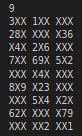
\includegraphics[scale = 0.8]{images/instance_2.png}
    \caption{Instance 1}
\end{figure}

First number determines the size of a puzzle; all subsequent lines correspond to one line of the puzzle. A 'X' means it is a clue to uncover. 

\section*{Z3 solving}

\textbf{Model:}\\

\begin{itemize}
    \item Let $X_{i,j} \in \{1..9\}$\footnote{Say $n=9$ to keep it simple.} be the value of the square at position $(i,j)$.\footnote{First line is top line; first collumn is left collumn.}
    \item Let $C$ be the clue set; a clue $c \in C$ is of the form $(i,j,v)$; where $(i,j)$ correspond to a position in the grid; $v \in \{1..9\}$
    \item $\forall (i,j,v) \in C: X_{i,j} = v$ \textbf{(Clues)}
    \item $\forall i, j, j' \in \{1..9\}, j \ne j' \Rightarrow X_{i,j} \ne X_{i,j'}$ \textbf{(Line Constraints)} 
    \item $\forall i, i', j \in \{1..9\}, i \ne i' \Rightarrow X_{i,j} \ne X_{i', j}$ \textbf{(Collumn Constraints)} 
    \item $\forall i,j,i',j' \in \{1..9\}, (i = i' [3]) \land (j = j' [3]) \land ( (i,j) \ne (i',j')) \Rightarrow X_{i,j} \ne X_{i', j'}$ \footnote{The 3 comes from $\sqrt 9$; understand $\sqrt n$ here.} \textbf{(Square Constraints)}
\end{itemize}

\textbf{Implementation details:}\\
The aformentionned model is implemented in \textbf{project.py}. The function \textit{line constraints} generates the constraints for the lines and the collumns; these being similar. \textit{integrity constraints} make sure every $X_{i,j}$ takes its value in $\{1..9\}$.\\
The functions \textit{str conversion} and \textit{int conversion} convert str types in int and vice versa. In the code, $X_{i,j}$ is an integer for Z3, but when we need to save it (or read the instance) we need to have a conversion tool. The utility of these functions becomes more obvious when we have $n > 9$. \\
Other functions are self-explanatory.

\textbf{Results:}\\



\section*{Presolve}



\end{document}